In this section we are going to report the results from simulations
for the Garbage Collector service described in Section
\ref{sec:gc_service}. The main problem that led to that solution was
the commit time of the Transaction State since it had to perform some
extra operations. The variables that were evaluated are the time to
commit a Transaction State object and the cluster utilization with and
without the Garbage Collector service. The simulations were conducted
in the first setup described earlier in this chapter.

\begin{figure}
\centering
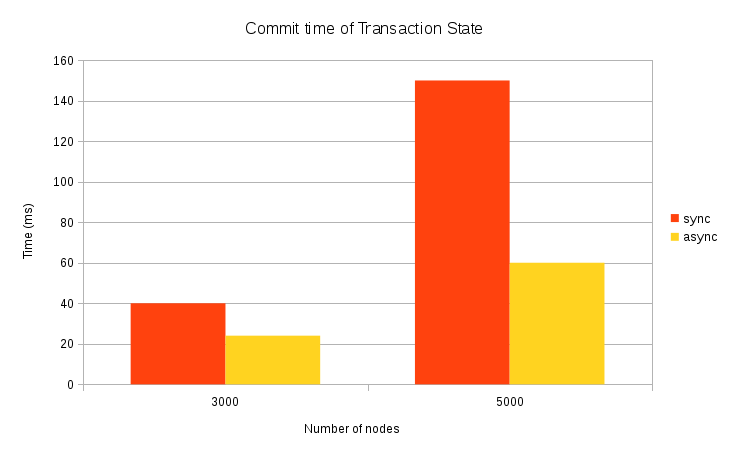
\includegraphics[scale=0.7]{resources/images/Evaluation/ts_commit_sync_async.png}
\caption{TS commit time with GC service}
\label{fig:ev_ts_sync_async}
\end{figure}

In Figure \ref{fig:ev_ts_sync_async} is depicted the total time taken
in milliseconds to persist the TS for 3000 and 5000 nodes in the
cluster. The time to commit affects both the scheduler and the
ResourceTracker regarding the updated view of the cluster and this has
a direct impact on the cluster utilization. For the simulation with
3000 NodeManagers the average commit time, even though it was already
low it dropped to 24 ms from 40 ms. The difference is more visible
for the simulation with 5000 nodes in the cluster where the commit
time dropped to 60 ms from 150 ms. In general we can observe a tension
to half the commit time and this is reasonable for several
reasons. First and foremost is because we do not have the foreign key
constraints in the tables that store RPCs (Figure
\ref{fig:impl_fk_yarn_rpc}). Also, the removal of old values is done
asynchronously so no overhead in the commit phase of the TS. Finally,
we have removed some \texttt{flush} operations from the application
logic that had to be there before to serialize the queries.


\begin{figure}
\centering
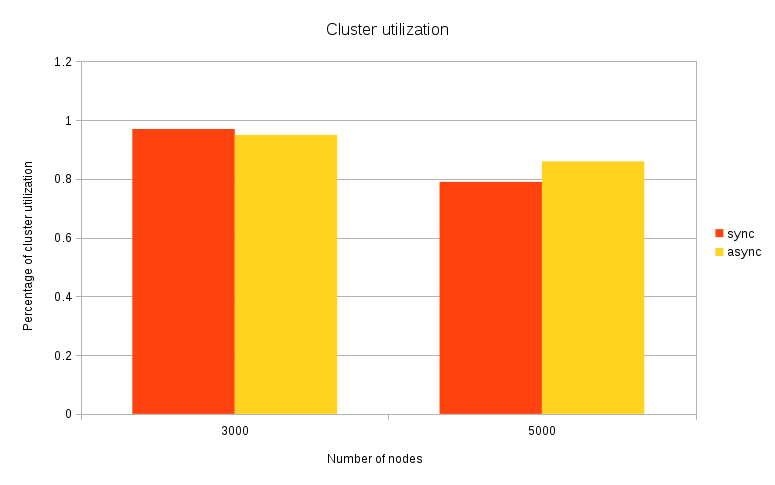
\includegraphics[scale=0.7]{resources/images/Evaluation/cluster_util_sync_async.png}
\caption{Cluster utilization with GC service}
\label{fig:ev_cluster_util_sync_async}
\end{figure}

The improvements on the commit time had a direct impact also in the
cluster utilization as we can see in Figure
\ref{fig:ev_cluster_util_sync_async}. For a 3000 nodes cluster the
utilization remained almost the same but it was already high
enough. Nevertheless, we have managed to improve the cluster
utilization by a few percentages for a 5000 nodes simulation, reaching
86 $\%$. The number of containers created in a 5000 nodes cluster
increased by 10$\%$ with the Garbage Collector service while in a 3000
nodes cluster it remained almost the same. Moreover, there is an interesting
side effect with decreased commit time. Since, TSs take less time to
commit, the blocking TSs that cannot be aggregated also spent less
time in the waiting queues of the Transaction Manager. That leads to
``smaller'' but more AggregatedTransactionStates. For instance, in the
simulation with 5000 NodeManagers without the GC service, there were
roughly 900 TS commits with on average 2000 objects to persist just
to update the status of NodeManagers. On the contrary, with the GC
service, there were 1690 TS commits with 960 objects to persist for
the NodeManagers. This side effect helped vanish the rollback of
transactions due to overloading (Section \ref{sssec:impl_aggr_new}), 
since there were not that many TSs in the queue to aggregate.